\chapter{Taking the plunge- The IMSc}

I knew Alladi Ramakrishnan the director of the Institute of Mathematical 
Sciences (IMSc). I had many friends there and I used to stop over there 
on my way to Kamuthi and give seminars.


As I have already said Alladi was a good teacher. He was a Professor in 
the old physics department of Madras University. The department was 
headed by the famous GN Ramachandran. Through the help of C Subramaniam 
who contacted Nehru who contacted Bhabha, Alladi founded IMSc. It is not 
easy to found an Institute. Full credit for that goes to him.


But whatever he did after that was not creditable. Apart from inviting 
famous physicists who happened to pass through India, he did nothing. He 
did not recruit active young physicists. His autocratic way of running 
the Institute did not attract good people. The institute consisted 
mostly of his own students. Once DAE came to know his mode of 
functioning, they cut the funds which added to his woes. He did not 
conduct proper selection committee meetings. Once a selection committee 
was announced. A selection committee member was stranded at the airport. 
Alladi prevented the meeting from taking place, by not sending the 
vehicle to the airport.

Even the faculty who were hired, were hired for 6 months or 3 months. 
His mode of functioning became worse after his son completed his studies 
and became a mathematician. After that Alladi's one-point programme was 
centered around his son only. I was a member of a selection committee 
convened by Alladi. MS Narasimhan was the chairman and Alladi's son 
Krishnaswamy was one of the candidates. When it was the turn of the 
committee to examine Krishna's case, we expected Alladi who was a member 
of the committee to withdraw. But he did not. The Chairman had to ask 
him to withdraw!
\eject

In 1983 I heard that the Director of IMSc, Alladi, was getting 
superannuated and he had to quit. But I never considered going to IMSc 
since it was worse than the University. It would be like jumping from a 
sinking ship onto a sinking boat. I had good contact with Udgaonkar and 
I had a good conversation with him on IMSc when we were in the same 
flight one day in 1983. A selection committee was set up to select the 
next director. Although I did not apply, the committee invited me for an 
interview. The Committee was chaired by V C Kulandaiswamy who had become 
the VC of the new Anna University. The other members were Udgaonkar and 
M S Narasimhan, the famous mathematician from TIFR. I went for the 
interview and I spoke frankly about the miserable state of IMSc and said 
if fresh blood could be infused, the Institute will survive.

I learnt that they had selected me. It was not clear to me whether I 
should be happy since I did not want to be an administrator although I 
did some administration as Head of the Dept in the University. I wanted 
to continue in physics.

Later I heard that ECG Sudarshan wanted to become Director and his 
friend Ramanna who was the Chairman of Atomic Energy Commission (AEC) 
decided to give the position to him. But apparently Sudarshan wanted 
also to hold his position in the University of Texas, Austin. So Ramanna 
wanted me to hold the fort at IMSc as a Deputy Director.

One day in 1983 I was informed that I must meet Ramanna. He was getting 
down from a military plane since he was the Defense Minister. I met him 
in the airfield itself. Ramanna said he had come only to meet me. Soon 
he was joined by Y S Das, the Additional Secretary. Both discussed the 
issue with me and tried to persuade me to accept the job. I was 
reluctant. The institute needed development and only a full-time 
Director can do it. How can I do it when the Director was sitting on the 
other side of the globe?

Later it seems that it was YS Das who solved the problem. Deputy 
Director cannot assume full powers. So they created the post of Joint 
Director and added this sentence in the constitution of IMSc: ``During 
the Director's absence the Joint Director shall have full powers of the 
Director".

Even then I was not very happy. Many of my friends (Virendra Gupta of 
TIFR, Kameshwar Wali of Syracuse University) who knew Sudarshan better 
advised me against the move. I was happy that Sudarshan's presence in 
Madras would brighten the academic atmosphere. I would have preferred 
his full-time presence as the Director of IMSc and I could continue in 
Madras University. Since I knew him as a friend, myself and others in 
the Department could derive considerable academic benefits. But that was 
not to be.

I knew Sudarshan well. My relationship with him was very good based on 
the high regard I had for him because of his top-class scientific 
achievement.In 1974 He invited me and my family to Austin, Texas. We 
spent two weeks there and he treated us like a royal family. Later 
during one of his Bombay visits, my high opinion came down a little 
because of the derogatory words he uttered about Mahatma Gandhi. My 
regard for him blinded me even to the wrong things about him that were 
said by others.

I got the appointment letter from the Tamil Nadu Government in October 
1983. But could not take a decision one way or the other. Meanwhile 
there was considerable pressure from DAE. Finally in February 1984, I 
took the plunge. There were five months between my receipt of the 
appointment letter and my acceptance of the job.

I went to the Institute and took charge from TD Sundararaj who was the 
Education Secretary of Tamil Nadu Government and who was officiating as 
the Director of IMSc. Alladi tried to extend his tenure by six months or 
at least by one month. But the Government did not give him even one day 
extra and made sure that Alladi really quits by asking Sundararaj to sit 
in the Director's chair!

%\section{Institute of Mathematical Sciences (1984-now)}

\section*{Building up IMSc (1984 to 1988)}

Once I decided to take up the job, I plunged into it with full force and 
commitment. When I joined, there were only 12 faculty members and 6 
students! Even after 20 years of existence the institute remained in the 
backwaters. Obviously recruitment was essential but that required many 
things to be done. Many developments had to take place. The following 
were taken up:
\begin{itemize}
\item Land for Hostel and Guest House, 
\item Central Government salary structure and other benefits, 
\item Recruitment of Faculty, 
\item Graduate School, 
\item MSc Programme (with Anna University), 
\item Theoretical Computer Science.
\end{itemize}

I will now describe how these were achieved. 

When I see how hard it has become to get additional land for IMSc, I 
realize how lucky we were in 1984. Since my first priority was to 
recruit faculty at an all-India level and an vibrant Graduate School and 
an active visitors' programme, it was clear that the zeroth order step 
was to get land for the Hostel and Guest House.

Once I eyed the piece of land opposite to IMSc, where buffaloes were 
grazing, I determined to go ahead and get it. The fact that I had good 
relationship with both C Aranganayakam who was the Education Minister of 
Tamil Nadu and the Chairman of our Governing Council and VC 
Kulandaiswamy who was the Director of Technical Education and a top 
Educationist, helped in the quick transfer of the land to us.

The salary-cum-allowance structure as well as other service benefits at 
IMSc were hardly such as to attract brilliant scientists to join here. I 
was keenly aware of the wide disparities that existed between IMSc and 
other national institutes where the salary structure was that of the 
Central Government.

In spite of many discussions and Committees that were set up, nothing 
tangible came out. At the end of my first year at IMSc, I was quite 
upset that we could not implement this measure which was a precondition 
for the success of our recruitment programme.

I decided to force the issue and worked out a strategy. I met Ramanna. 
He was sympathetic and appreciated the need for prompt action. He agreed 
to sign the letter (drafted by me) addressed to Aranganayakam. I carried 
the letter personally to the Minister and explained the situation to 
him. His approval was very prompt and I knew that day that the battle 
was won. I announced the improved service benefits to the Faculty 
immediately. This was the way the Gordian knot of Committees and 
Subcommittees was cut.

There were still some hitches. For instance the administrative and 
service staff was still not covered by the new scheme. I took our 
Registrar G Sethuraman with me to meet Ramanna at Kalpakkam to convince 
him of the advisability of enlarging the scheme to the administrative 
and service staff.

As a result of these endeavours, all the obstacles were removed and our 
recruitments started in full swing. Of course the benefits were 
applicable to everybody, whether new recruits or existing members. Every 
member of IMSc got a substantial increase in his or her pay with 
retrospective effect. Many other welfare measures available in other 
central government institutions such as Leave Travel Concession, Medical 
Scheme could be implemented in IMSc soon after, since all these were 
regarded as part of the same package.

Further, once the status of the IMSc members to be on par with others 
governed by the central government system was granted, then the 
subsequent improvements recommended by the Pay Revision Commissions 
became automatically applicable to our members. These benefits are 
enjoyed by all of us now, thanks to the government of Tamil Nadu and 
DAE.
\smallskip

During these four years (1984 to 1988), the faculty strength grew from 
12 to 31. Both in Theoretical Physics and Mathematics we were able to 
attract very brilliant young people who became the pillars of IMSc in 
the subsequent years.
\smallskip

The close contacts that I had with various Centres in the country where 
good Theoretical Physics groups existed and similar contacts and even 
more importantly the stature that Seshadri enjoyed among mathematicians 
facilitated the recruitment programme. In fact most of the new faculty 
members in Theoretical Physics were known to me academically and all the 
new faculty members in Maths were known to Seshadri academically.
\smallskip

Along with the new faculty expansion, we recruited a large number of 
research students also. The total number of post-doctoral research 
fellows and research students increased from 6 to 35 in two years.
\smallskip

An important feature of the new recruitments must be stated and stressed 
here. In contrast to the original composition of IMSc before 1984 which 
consisted predominantly of members from a single state only, the newly 
recruited faculty and students hailed from various states spread all 
over the country. Thus IMSc achieved a truly national character.
\smallskip

Systematic post-MSc level courses for the research students working 
towards their Ph D degrees were started during this period, in all 
subjects coming under Theoretical Physics and Maths, since a sizeable 
number of students had joined as already mentioned.
\smallskip

Jagannathan and myself prepared detailed syllabi in all the subjects 
under Theoretical Physics. Jagannathan's keen interest in teaching and 
especially the meticulous care to detail that characterized all his work 
played a major role in putting the teaching of theoretical physics on a 
sound track. We thus laid the foundation for the Graduate School at IMSc 
that has flourished over the years.
\smallskip

From early on, it was clear to me that there was a serious gap in our 
graduate school. Although the School was primarily intended for post-MSc 
students, we had allowed ``exceptionally bright" post-BSc candidates also 
to apply. In fact there were a few who had only BSc, but were better than 
the best post-MSc students. It seemed a pity to send them back to 
college for another two years for getting an MSc degree.
\smallskip

I discussed this problem with VC Kulandaiswamy who had become the VC of 
the newly created Anna University. He had also appointed me as member of 
the Syndicate, Academic Council and the Board of Studies of the 
University.
\smallskip

He understood the issue and agreed to introduce a new degree called MSc 
(by research) in the University that can be run by IMSc faculty in 
collaboration with Anna University. Since I had been inducted into all 
University bodies it was possible for me to discuss with members of all 
of them and get the new degree approved.
\smallskip

This is how MSc started at IMSc and it functioned as a door to introduce 
``exceptionally bright" candidates into research, just after their BSc 
degree.
\smallskip

Starting of Theoretical Computer Science Research is another milestone 
in the growth of the Institute during 1984-88. In the pre-1984 period 
there was no Theoretical Computer Science group in IMSc. Such a group 
was formed after PS Thiagarajan joined IMSc in 1986. Soon other younger 
members joined and a strong TCS group has been flourishing at the 
institute.
\smallskip

Although I had full powers I knew about Sudarshan's ego. So I made it a 
point to discuss with him when he came after his stay in Texas, all the 
important steps taken by me and got them signed by him. In the beginning 
things went on smoothly. In fact many times he told me ``Rajasekaran, we 
seem to be thinking along the same lines!"
 
But as the years went by, things changed.

\section*{Turmoil(1989)}

Sudarshan spent less and less time at IMSc during the four years 84-88. 
Every year he spent half the year in Austin, Texas. Some years it was 
more. This would not have mattered much if the Joint Director had been 
allowed to function with full power. But Sudarshan's ego prevented that. 
Slowly he began to dislike everything I had done in his absence. He 
would come after a long break and make decisions inconsistent with what 
was done in his absence.

More importantly, selection of faculty was being held up. It was very 
difficult to have Selection Committee meetings during the period of his 
brief presence since other members who were busy could not come on those 
days.

Especially in Mathematics this became a serious issue. Seshadri insisted 
that I must act since I had the authority. So I conducted a Selection 
Committee meeting in Sudarshan's absence. M R Srinivasan was in the 
chair. I sent out the appointment letters. When Sudarshan learnt about 
this he was furious. I told him it was a duly appointed selection 
committee and I had authority to hold its meeting.

One of the candidates selected was V S Sundar, a mathematician. He 
joined. Sudarshan called him to his office and told him point-blank that 
he must quit since his appointment is cancelled. This must be an 
unprecedented behavior by the Director of any institution. Sundar left 
and rejoined only after Sudarshan was removed. He has done high-quality 
mathematics ever since.

IMSc had one faculty member representing the faculty in the Governing 
Council. So far KR Unni, was doing that and his term ended. Whom to 
appoint now? Earlier I think Alladi simply did it by fiat. I thought of 
doing it more rationally. There were two candidates, ND Haridass and 
Seshadri. Although I preferred Seshadri I decided there shall be an 
election. Seshadri was chosen unanimously. That also angered Sudarshan.

I must say something more about Seshadri here. From the beginning it was 
clear that Seshadri, being an eminent mathematician and involved in the 
actual recruitment of mathematical faculty in IMSc, must be made 
in-charge of the Maths group. This simple thing was resisted by 
Sudarshan. He wanted to play politics between Unni and Seshadri by not 
announcing that Seshadri was in-charge of the maths group.

Meanwhile Seshadri became FRS. It became a glaring injustice not to make 
him in-charge of the Maths group.

As for my relations with Alladi, in the beginning they were cordial. 
In fact after hearing that I was to take over, he threw a party to 
welcome me! The relationship got soured only because of his son. 
Krishna, while being on the rolls of IMSc as a faculty member, was 
almost permanently abroad. Once when his application for extending his 
leave came to me as the director-in-charge, I refused. Alladi himself 
phoned me repeatedly asking me to grant his son's application. I had to 
cut him short. From that time Alladi treated me as his enemy.
 
All these things accumulated increasing the tension in the Institute. 
But the event that toppled the apple cart is the dismissal of 
Sethuraman, our registrar. In the beginning years at IMSc I had 
struggled with the administration and I felt that a competent registrar 
is necessary. I went to Ramanna for help. He sent G Sethuraman from DAE 
as our registrar. I knew him since earlier he was the typist cum 
secretary in the Theoretical Section of TIFR. In fact many of my papers 
intended for publication were typed by him. He turned out to be an 
excellent registrar having good liaison with DAE.

Above all Sethuraman had unquestionable integrity. So he did not like 
some of the money dealings of Sudarshan which were shady and apparently 
will involve the institute also. Sethuraman expressed his misgivings to 
Sudarshan. The latter dismissed the former unceremoniously without giving 
any reason.

That was too much. I had to act. I sent a detailed report to M R 
Srinivasan who was the Chairman of the Governing Council (GOC) with 
copies to all the members. In the main I mentioned the continued absence 
of Sudarshan for months together and his erratic actions when he comes. 
I said I cannot hold the fort under these circumstances. Actually this 
is the first time that the GOC became aware of Sudarshan's absence from 
IMSc for long periods.

Sudarshan's reaction was violent and became more erratic. He cut off my 
official phone connection. He gave a kick to the door of my office room 
and removed my name plate.

I felt even my life to be in danger and wanted to be away from Madras. 
Both IIT Kanpur and IIT Bombay offered me refuge. The former sent me the 
appointment letter. Finally I decided to go to TIFR, vowing to return 
only after Sudarshan was removed. TIFR was a familiar place for me. Also 
I could watch what DAE was going to do.

In this struggle, most of the faculty supported me. In particular, there 
were Haridass, Baskaran, Thiagarajan and Balasubramaniam who were with 
me. Of course Seshadri was with me. Only the faculty who joined before 
1984 did not support because of their alleged loyalty to authority.

Thanks to TIFR I enjoyed peace for one year (1989). There I could return 
to Physics and complete some of the research projects.

Finally Sudarshan left at the end of 1989. He had to leave since his 
5-year term ended. But he went to the court against the institute 
claiming he was a permanent director. He quoted some statement of Indira 
Gandhi the Prime Minister as evidence. But he had signed a 5-year 
contract. He tried to hide that, but Sethuraman managed to unearth it 
and the judge threw that at his face and dismissed the case. Of course 
all this took time.

My sufferings were not over. He filed a criminal case against me citing 
the official letter I had written to the GOC as defamation. I had to 
fight it out. My lawyer told me that according to Indian law, if you 
call me a fool it is not defamation if you can prove it. So the 
lawyer asked the court to ask Sudarshan to produce his passport which 
will prove his absence. His lawyer went on asking for postponement for 
many months. My lawyer had advised me to be present whenever my case 
came up. His lawyer did not appear at all. So finally the judge 
dismissed the case.

All this took time, also money. Sudarshan could throw away a few dollars 
at his lawyer, but in my case it was my hard-earned money. Later IMSc 
offered to reimburse this expense, but I was not keen. Sudarshan's aim 
was only to torture me and he succeeded.

Let me mention two unexpected fall-outs from the turmoil.

Prof Seshadri left IMSc with a group of Maths and TCS people and founded 
what became known as CMI (Chennai Mathematical Institute). Thus a good 
thing can emerge from a bad happening!

A very strong group of high-energy-physicists, Anjan Joshipura, Saurabh 
Rindani and Utpal Sarkar, whom I had hired left IMSc during the turmoil 
and founded the HEP group at the Physical Research Laboratory 
(PRL), Ahmadabad. What was a loss for IMSc became a gain for PRL!

\section*{Back to peace and progress (1990-now)}

The Institute was put back on the path of progress in 1990. R 
Ramachandran took over as Director in 1990 and IMSc had a smooth sail 
after that. Thanks to him I could get back to academic activity. During 
his term and after Balasubramaniyam took over in 2000, the institute 
continued to grow and has reached great heights. Progress continues with 
the present Director V Arvind.

\begin{figure}[H]
\centering
\includegraphics[width=0.9\textwidth]{images/new-images/08-Rajaji-fest.jpg}
\caption{The attendees of my 65th birthday function (Rajaji Fest)}
\end{figure}

The following event might have happened in 2011 when the Golden Jubilee 
of IMSc was celebrated. The famous physicist David Gross who is a Nobel 
Laureate visited the Institute and went to Kolkata. I was also going to 
Kolkata and so we traveled together. His wife was with him. At the 
Chennai airport he wanted to wait at the VIP's lounge and wanted me also 
to be with him. In the lounge, there was Amartya Sen, another Nobel 
Laureate with his wife. Gross and Sen knew each other. So, for a while I 
was enjoying the company of two Nobel laureates!

But the story does not end there. After the plane took off, Gross came 
to me running and said ``Rajaji, I lost my laptop in the airport." At the 
security check-up he forgot to pick it up. Although the laptop was an 
expensive one, he was particularly worried since he had many valuable 
documents in that laptop. After we landed, from the Kolkata airport 
people it was difficult to get any help. Fortunately my friend R Simon 
from IMSc happened to have arrived at Kolkata airport at the same time. 
With his authoritative voice and gestures, he forced the airport people 
to make the connection to the Chennai airport. We got the news that the 
laptop is safe and will be sent to Gross in USA. Gross did receive it in 
due time.

\begin{figure}[h]
\centering
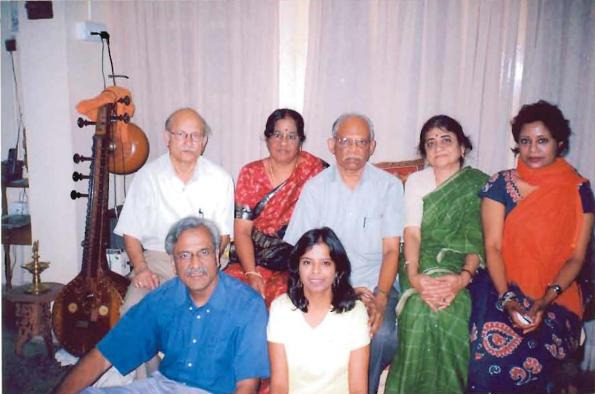
\includegraphics[width=0.9\textwidth]{images/Rajaji-family.jpg}
\caption{ L to R: Rajat Bhaduri, Suthandra, GR, Manju Bhaduri, Poongodhai.
Below: MVN Murthy, Uma.}
\end{figure}

\medskip

%~ \begin{figure}[h]
%~ \centering
%~ 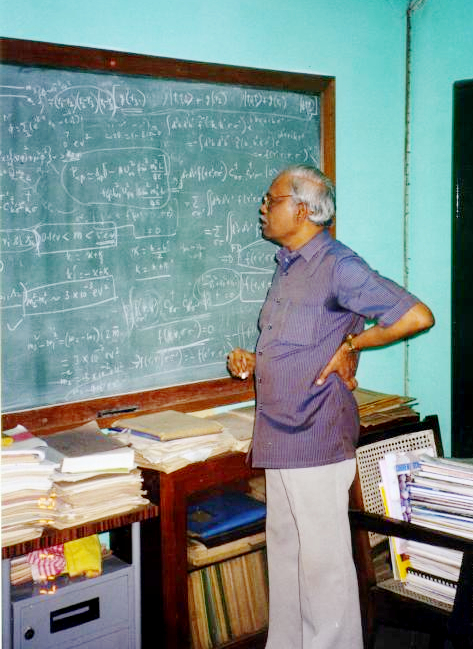
\includegraphics[width=.6\textwidth]{images/rajaji1.jpg}
%~ \caption{At the blackboard in my old office.}
%~ \end{figure}

